\documentclass[journal,twoside,web]{ieeecolor}
\usepackage{generic}
\usepackage{cite}
\usepackage{amsmath,amssymb,amsfonts}
\usepackage{algorithmic}
\usepackage{graphicx}
\usepackage{algorithm,algorithmic}
\usepackage{hyperref}
\hypersetup{hidelinks=true}
\usepackage{textcomp}
% added packages
\usepackage{subcaption}
\graphicspath{{Fig/}}
\usepackage{booktabs}
\usepackage[flushleft]{threeparttable}
\usepackage{placeins}
%\usepackage{natbib}
\usepackage{subcaption}
\graphicspath{{Fig/}}
\usepackage{booktabs}
\usepackage[flushleft]{threeparttable}
\usepackage{placeins}


\def\BibTeX{{\rm B\kern-.05em{\sc i\kern-.025em b}\kern-.08em
    T\kern-.1667em\lower.7ex\hbox{E}\kern-.125emX}}
\markboth{\hskip25pc IEEE TRANSACTIONS AND JOURNALS TEMPLATE}
{Author \MakeLowercase{\textit{et al.}}: Title}
\begin{document}
\title{DruGNNosis-MoA: Elucidating Drug Mechanisms as Etiological or Palliative With Graph Neural Networks Employing a Large Language Model}
\author{Brettler Liad, 
Berman Eden,
Jagodnik Kathleen M.,
and 
Bartal Alon
%\thanks{This paragraph of the first footnote will contain the date on 
%which you submitted your paper for review. It will also contain support information, including sponsor and financial support acknowledgment. 
%For example, ``This work was supported in part by the U.S. Department of Commerce under Grant 123456.'' }
\thanks{
All authors are with the The School of Business Administration, Bar-Ilan University, Ramat-Gan, 5290002, Israel (e-mail: alon.bartal@biu.ac.il).}
%\thanks{Second B. Author Jr. was with Rice University, Houston, TX 77005 USA. He is 
%now with the Department of Physics, Colorado State University, Fort Collins, 
%CO 80523 USA (e-mail: author@lamar.colostate.edu).}
%\thanks{Third C. Author is with 
%the Electrical Engineering Department, University of Colorado, Boulder, CO 
%80309 USA, on leave from the National Research Institute for Metals, 
%Tsukuba, Japan (e-mail: author@nrim.go.jp).}
}

\maketitle

%Full names of authors are preferred in 

%the author field, but are not required.

%Put a space between authors' initials.

%The abstract must be between 150--250 words. 

% three or four different keywords or phrase

\begin{abstract}
Understanding the complex mechanisms of drugs' therapeutic effects is essential for advancing precision medicine and optimizing treatment strategies. 
However, systematically distinguishing between drugs that address root causes (etiological mechanisms) and those that alleviate symptoms (palliative mechanisms) using modern Artificial Intelligence (AI)-based strategies remains underexplored.
We present a novel computational framework for classifying drug Mechanisms of Action (MoA) as etiological or palliative, comparing three models: 
(i) fine-tuning Science Bidirectional Encoder Representations from Transformers (SciBERT) with drug descriptions; 
(ii) training a Graph Neural Network (GNN) model on a constructed heterogeneous network of drugs, genes, and diseases; and 
(iii) developing DruGNNosis-MoA, which integrates GNN with our fine-tuned SciBERT embeddings as node features. 
DruGNNosis-MoA excelled (F1-score 0.94) in identifying drug MoA. 
DruGNNosis-MoA characterizes drug mechanisms for subsequent pharmacological studies, thereby advancing precision medicine and therapeutic development.
\end{abstract}

\begin{IEEEkeywords}
%alphabetical order, separated by commas.
Etiological drugs;
Graph Neural Network (GNN);
Large Language Model (LLM);
Palliative drugs
\end{IEEEkeywords}

%======================
\section{Introduction}
\label{sec:intro}
%======================

% Challenges in Developing New Drugs
\IEEEPARstart{M}{odern} medicine uses pharmaceutical interventions to combat diseases, alleviate symptoms, and support recovery through non-invasive treatment \cite{ravikumar2018improving,yu2020exploring}.
However, developing a new drug in the pharmaceutical industry is often prolonged, resource-intensive, and prone to frequent failures \cite{hammel2019new,xue2018review}.
Indeed, a considerable number of drug development initiatives fail to secure approval for public use, with critical issues frequently emerging at later stages of the drug discovery process \cite{hammel2019new}.
Preventing adverse reactions, balancing efficacy and toxicity, enhancing drugs, and addressing legal and financial factors add complexity to drug approval \cite{ravikumar2018improving}.

% Description of etiological and palliative drug mechanisms
Drugs can either directly target the underlying disease cause, or focus on alleviating a disease's symptoms \cite{yildirim2007drug,lindpaintner2002impact}.
Improving the drug design process can be informed by expanding our comprehension of these two fundamental drug mechanisms: 
(i) etiological -- targeting the root causes or contributing factors of a disease, and 
(ii) palliative -- alleviating symptoms by targeting proteins not directly implicated in the primary cause but involved in counteracting the disease's effects \cite{yildirim2007drug,lindpaintner2002impact}.
This distinction in drug mechanisms could guide the development of precise treatment strategies, minimizing side effects, optimizing resource allocation, and facilitating evidence-based healthcare decisions tailored to individual patients \cite{vogt2014molecularly}. We note the distinction between the broad concept of drugs with palliative mechanisms, used to treat the general population, which drugs are the focus of the current project, vs. the narrower concept of drugs used specifically for end-of-life care, termed 'palliative' care, which typically employs opioids, anticholinergics, antipsychotics, and benzodiazepines for symptom relief during terminal illness \cite{jansen2018safety}.

% The difficulty in classifying drugs as etiological and palliative.
Distinguishing between etiological and palliative mechanisms of action (MoAs) involves challenges due to the complex nature of disease processes, potential overlap between targeting root causes and symptom relief, dual mechanisms exhibited by some drugs, limited treatment options for specific conditions, patient variability, the rarity of many diseases and conditions, and the interdisciplinary nature of healthcare \cite{yu2020exploring}.
The comprehensive classification of drugs based on MoAs is an under-studied aspect of drug research, motivating this study.

% Drug repurposing potential
The discovery of new drugs can also arise from drug repurposing \cite{parvathaneni2019drug}.
This involves identifying shared mechanistic characteristics among approved drugs, spanning related and additional Anatomical Therapeutic Chemical (ATC) classes \cite{xue2018review}.
Within the ATC classification system, active substances are grouped based on specific target organs or systems, as well as therapeutic, pharmacological, and chemical characteristics.
Leveraging the ATC classification facilitates the identification and exploration of potential drug treatments for new or under-studied diseases \cite{yang2017literature}.
For instance, \cite{olson2017predicting} utilized the ATC system to identify novel drug treatments for unstudied diseases.

% Prior work, introducing Lindpaintner and Yildirim
The systematic examination of etiological vs. palliative drug MoAs has received limited attention \cite{yildirim2007drug,lindpaintner2002impact,guney2016network}.
\cite{lindpaintner2002impact} provided examples to delineate this distinction, while \cite{yildirim2007drug} constructed networks that assessed drugs' proximity to diseases via protein interactions, and revealed an enrichment of palliative drugs.
Additionally, \cite{yildirim2007drug} suggested using the shortest distance between drug-target proteins and disease-gene product proteins as an indicator to classify drugs based on the molecular steps between a drug target and its associated disease cause.
Hence, short network distances between proteins indicate etiological mechanisms, while long distances suggest palliative mechanisms. 
More recently, network analysis was used for drug screening \cite{guney2016network} that employs a drug-disease proximity measure quantifying relationships among drug targets and diseases, and assessing to what degree each drug is palliative vs. `effective'. 

% Other studies on different drug mechanism classification (literature review)
Numerous studies \cite{thafar2020dtigems+, sachdev2019comprehensive,vogt2014molecularly} of drug research and development have overlooked the crucial distinction between etiological and palliative mechanisms, neglecting the utilization of extensive datasets and contemporary analytical methods, such as Machine Learning (ML).
Other studies often focus on predicting drug-target interactions, repurposing \cite{fahimian2020repcool}, or drug mechanisms, lacking systematic classification \cite{vogt2014molecularly}.

% The opportunity available today to study these mechanisms using ML
Recent technological advances including the use of large-scale experimental validation of protein interactions, identification of disease-associated genes, and ML models, can aid in the field of drug discovery.
For example, a Graph Neural Network (GNN) is an ML model that captures the inherent qualities of a graph by transferring information between its nodes \cite{zhou2020graph}.
GNNs are effective for capturing complex patterns and dependencies in relational data.
Additionally, GNNs have been reported as highly effective in various graph analysis tasks, including node classification, link prediction, and graph clustering \cite{bongini2021molecular,jiang2021could,zhou2020graph}.
Leveraging the network's inherent structure, GNNs hold significant promise for revealing latent patterns and connections involving drug MoAs, facilitating the classification of drugs as having etiological or palliative MoA.

% Presenting three classification models
Aiming to differentiate drugs with etiological vs. palliative mechanisms, we leveraged three extensive biomedical datasets, performing a comprehensive investigation of 2,018 U.S. FDA-approved drugs.
We developed three classification models:
(i) fine-tuned a Science-BERT (SciBERT) model -- a Large Language Model (LLM) that was pre-trained \cite{beltagy2019scibert} on drug descriptions from DrugBank \cite{wishart2018drugbank,knox2024drugbank};
(ii) trained a GNN model \cite{huang2020combining}; and
(iii) trained a GNN model with textual node features extracted from drug descriptions processed by a fine-tuned SciBERT model, resulting in numerical embeddings.

% Goal and motivation
Our study innovates by employing advanced ML techniques to analyze extensive and diverse biomedical datasets for the elucidation of etiological and palliative drug mechanisms.
The systematic exploration of these mechanisms not only promises a paradigm shift in understanding drug actions but also holds the potential to reshape the landscape of early-stage drug discovery, refine personalized treatment selections, and optimize drug repurposing strategies.

%----------------------------------------------------------------------
\section{Related Work}
%----------------------------------------------------------------------
Drug classification based on etiological vs. palliative mechanisms of action has not been systematically researched using the most current available computing strategies.
To our knowledge, there has not yet been a model developed that categorizes drugs as etiological or palliative that employs Graph Neural Networks (GNNs) or Large Language Models (LLMs).
\cite{yildirim2007drug} proposed that in their network, distances greater than 1, which mirrored results from a randomized network, could be indicative of palliative drugs, while distances of 0 and 1, showing statistical significance, might represent etiological drugs.
Their findings suggest a prevalence of palliative drugs, with a smaller proportion of etiological ones.
\cite{yildirim2007drug} also speculated that future developments might lead to a rise in the number of etiological drugs.
Our research seems to validate this prediction.
\cite{yildirim2007drug}'s paper anticipated a growth in the development of etiological drugs, a hypothesis we explored in this paper.
However, we observed a limitation in \cite{yildirim2007drug}'s approach of classifying drugs based solely on the shortest distances within the network.
While trying to replicate their methodology, we could not find significant correlation between drug mechanisms and network distance.
Both types of drug mechanisms appear in short and long network distances. 
Furthermore, their work lacked a detailed explanation of the methodology used to calculate these shortest distances, particularly concerning the selection of drug-disease pairs.
To address these gaps, our study has investigated three distinct analytical strategies to calculate drug-disease distances, as shown in Fig. S5, %\ref{fig:yildirim}, 
providing a more nuanced understanding of drug classification in the context of etiological and palliative mechanisms.

%\begin{center}
%[Figure \ref{fig:yildirim} about here.]
%\end{center}

The All vs. All (Comprehensive) Method examines all possible paths between each drug and disease pair.
These results, as depicted in Fig. S5a%\ref{fig:yildirim1}
, exhibit the most resemblance to \cite{yildirim2007drug}'s findings \cite[Figure~6a]{yildirim2007drug}.
When excluding instances of drug duplicates from the same distance, using the All vs. All (Unique) Method depicted in Fig. 5b,%\ref{fig:yildirim2}, 
the distribution of drug mechanisms is proportional at each distance value.
This indicates that almost every drug has a corresponding disease at each distance.
We believe that the Unique Minimum Shortest Distance Method, shown in  Fig. S5c, %\ref{fig:yildirim3}, 
offers the most insightful analysis.
This method reveals a significant concentration of connections at distances 0 and 1, aligning with \cite{yildirim2007drug}'s observations of statistical significance.
However, contrary to \cite{yildirim2007drug}'s suggestion, this method demonstrates a combination of etiological and palliative drugs within each distance.
For example, at distance 1, there are 218 etiological drugs and 136 palliative drugs.
This challenges the notion that distances $> 1$ predominantly represent palliative drugs.

More recently, \cite{guney2016network} analyzed large-scale datasets via network analysis to develop a drug-disease proximity measure to quantitatively assess the distances between drug targets and diseases, and categorize drugs as palliative or 'effective' (compared with our terminology of 'etiological'). They concluded that their metric provides an unbiased measure of the therapeutic effects of drugs that permits the differentiation of 'causative' ('effective') treatments from palliative ones. This team reported that their network-based framework improves upon existing drug repurposing approaches, including similarity-based methods. As in our work presented here, \cite{guney2016network} assessed the Anatomic Therapeutic Chemical (ATC) classifications of proximal and distant drug-disease pairs and presented trends identified in these analyses.

%=========================================================
\section{Data}
\label{sec:materials}
%=========================================================
\subsection{Drug-Target Data}
\label{sec:DrugBank_data}
%-------------------------------------------------------
Using drug and gene target information from DrugBank (Version 5.1.10) \cite{wishart2018drugbank}, we recorded FDA-approved drugs targeting human genes, excluding those affecting retroviral genes. This process resulted in 2,018 drugs connected to 2,232 gene targets.
Drugs are represented by chemical IDs, and genes are represented by GenBank \cite{benson2012genbank} protein IDs and names.

%-------------------------------------------------------
\subsection{Protein–Protein Interaction (PPI) Data}
\label{sec:PPI_data}
%-------------------------------------------------------
We gathered experimentally validated PPIs in humans from the `Non-redundant' BioGRID database (Version 4.4.217) \cite{oughtred2021biogrid}.
We regard each interaction between protein \textit{A} and protein \textit{B} as bidirectional.
Identical interactions captured using a different experimental system or publication source were eliminated.
Proteins are represented by their official interactor gene symbols (i.e., gene names).
Hereafter, the proteins associated with genes are termed genes.
To ensure dataset coherence, we included only human genes, excluding PPIs associated with retroviruses.
The final dataset comprises 781,272 gene-gene interactions involving 19,893 genes within the human genome.

\subsection{Disease-Gene Data}
\label{sec:OMIM_data}
Information on the relationships between genotype and disease phenotype in humans was gathered from the Online Mendelian Inheritance in Man (OMIM) Morbid Map dataset (downloaded May 1, 2023) \cite{amberger2015omim}.
The dataset comprises OMIM's Synopsis of the Human Gene Map, encompassing 8,156 diseases and 16,358 disease-associated genes.
Diseases are represented by their phenotype name, while genes are represented by gene symbols.

%======================================================================================
\section{Methods
}\label{sec:methods}
%======================================================================================

\subsection{Drug Mechanism Labeling}
\label{sec:annotation}
%---------------------------------------------------------------------------------
Analyzing drug therapeutic mechanism information in DrugBank, we focused on the Identification and Pharmacology fields and manually classified each drug as having etiological, palliative, or both mechanisms. Each drug was annotated (Supplementary Table S1) by two independent annotators having bioinformatics training. 
In the case of conflicting labels, the discrepancy was discussed to achieve agreement on the final annotation.
This manual evaluation yielded an annotated dataset that delineates the mechanism of each drug.
For example, addressing vitamin deficiency, interventions such as replacement therapy or induced secretion of the deficient vitamin were classified as etiological, while drugs for alleviating the symptoms of the deficiency were labeled as palliative.

\subsection{Fine-tuning SciBERT}
\label{sec:SciBERT}
We fine-tuned the SciBERT language model \cite{beltagy2019scibert} for classifying drugs as etiological or palliative using drug descriptions from DrugBank and drug labels.
The training data included text from the Pharmacodynamics and MoA sections in DrugBank, with explicit indications of etiological or palliative mechanisms manually omitted to ensure that the model learned from a general context. 
The dataset was split into 90-10\% Training-Testing sets, with the Training set further divided into a 10\% Validation set. 
We employed a 10-fold cross-validation (CV) for fine-tuning SciBERT and assessed its performance using the F1-score.
The best model, selected during CV, was then evaluated on the Test set.

\subsection{Network Modeling}
\label{sec:networks}

To reveal the complex relationships among diverse biological and pharmaceutical elements, we constructed four networks using the NetworkX Python package \cite{SciPyProceedings_11}.

%---------------------------------------------------------------------------------
\subsubsection{Network Construction}
\label{sec:network_construction_1}
%---------------------------------------------------------------------------------
\textbf{Drug-Target Network.}
Associates drugs and their target genes utilizing DrugBank data.
Designed as a bipartite graph, nodes correspond to drugs or target genes.
The network's links signify instances where a drug targets a specific protein translated from its associated gene.

\noindent\textbf{Protein-Protein Interaction (PPI) Network.}
Associates human proteins within a biological system based on BioGRID data.
Proteins are gene nodes, and two proteins are linked if a genetic interaction is reported.

\noindent\textbf{Disease-Gene Network.}
Associates diseases with their associated genes within OMIM Morbid Map.
Designed as a bipartite graph, nodes signify genes or diseases, and network links denote known associations between a gene and a disease.

\noindent\textbf{Heterogeneous Network.}
Using the Drug-Target, PPI, and Disease-Gene networks, we constructed a heterogeneous network.
To facilitate binary classification, drugs displaying a dual role of both etiological and palliative mechanisms were excluded, and are reserved for future use.
We utilized the heterogeneous network for the development of two GNN models.
Nodes of the heterogeneous network represent drugs, genes, and diseases.
Each drug node has a label attribute indicating either etiological or palliative mechanism.
Links (edges) of the heterogeneous network include: drug-gene (targeting), gene-gene (protein interaction), and disease-gene (association).
Next, we trained a GNN model using the PyTorch Geometric (PyG) library with our heterogeneous network \cite{Fey/Lenssen/2019}.

%-----------------------------------------------------------
\subsubsection{Graph Neural Network Model Development}
\label{sec:model}
%-----------------------------------------------------------
Since GNNs excel in node classification by learning complex characteristics from graph structures, we trained two GNN classifiers on our heterogeneous network: Baseline GNN, and the DruGNNosis-MoA as described in the next paragraphs. 
To enhance the developed GNN's learning capability, we incorporated two SAmple-and-aggreGatE (SAGE) Convolution layers (SAGEConv) \cite{hamilton2018inductive} from the PyTorch Geometric (PyG) Python library \cite{Fey/Lenssen/2019}.
Using the Rectified Linear Unit (ReLU) activation function \cite{shang2016understanding} for non-linear pattern capture and a Sigmoid function \cite{vlačić2020neural} for binary predictions, we employed the Adam optimizer \cite{kingma2014adam} for weight adjustments during training. 
%This forms the foundation for developing two GNNs.

\textbf{Baseline GNN.}
Given the heterogeneous network, we assign the EigenVector decomposition for each node \cite{huang2020combining}.
The EigenVector captures informative features for each node.
Next, we standardized the EigenVectors (Z-score normalization) for subsequent analysis.

\textbf{DruGNNosis-MoA.}
Given the heterogeneous network, we integrated textual features (embeddings) for each node.
To generate textual node features, we applied the fine-tuned SciBERT model on drug descriptions from DrugBank; gene symbols from PPI data; and disease names from OMIM.
We then reduced the dimensionality of text embeddings from the fine-tuned SciBERT model to size 128 using Principal Component Analysis (PCA), thus enhancing the foundational feature input for the DruGNNosis-MoA model.
This reduction focuses the model on the most relevant aspects of the data.


%-----------------------------------------------------------
\subsubsection{Graph Neural Network Training}
\label{sec:Train}
%-----------------------------------------------------------
We divided drug nodes into Train (90\%) and Test (10\%) sets, implementing a 10-fold CV on the Train set, reserving 10\% of the Train set as a Validation set in each fold.
Both the partitioning and CV were conducted in a stratified manner, ensuring a balanced and proportional distribution of each label class and mitigating the risk of biased model training.
We applied a transductive node classification approach, enabling all sets to access the complete graph structure.
However, they were limited to knowing only the labels of the nodes within their respective subsets.

%-----------------------------------------------------------
\subsection{Model Evaluation}
%-----------------------------------------------------------
To ensure a fair comparison among the fine-tuned SciBERT; the Baseline GNN; and the DruGNNosis-MoA models in terms of MoA classification, we used the same 10-fold CV process to evaluate their performances.
The average cross-validation metrics, including F1-score, recall, precision, and area under the curve (AUC), were reported for each model.
To determine the best-performing model, we compared the averages F1-scores and ROC-AUC scores across the three models.
Finally, the performance of the selected best model was evaluated on the Test set using the same metrics.

Fig. \ref{fig:FlowChart} summarizes the methods employed in this study.
\vspace{-3.5em}
\begin{figure}[H]
    \centering
    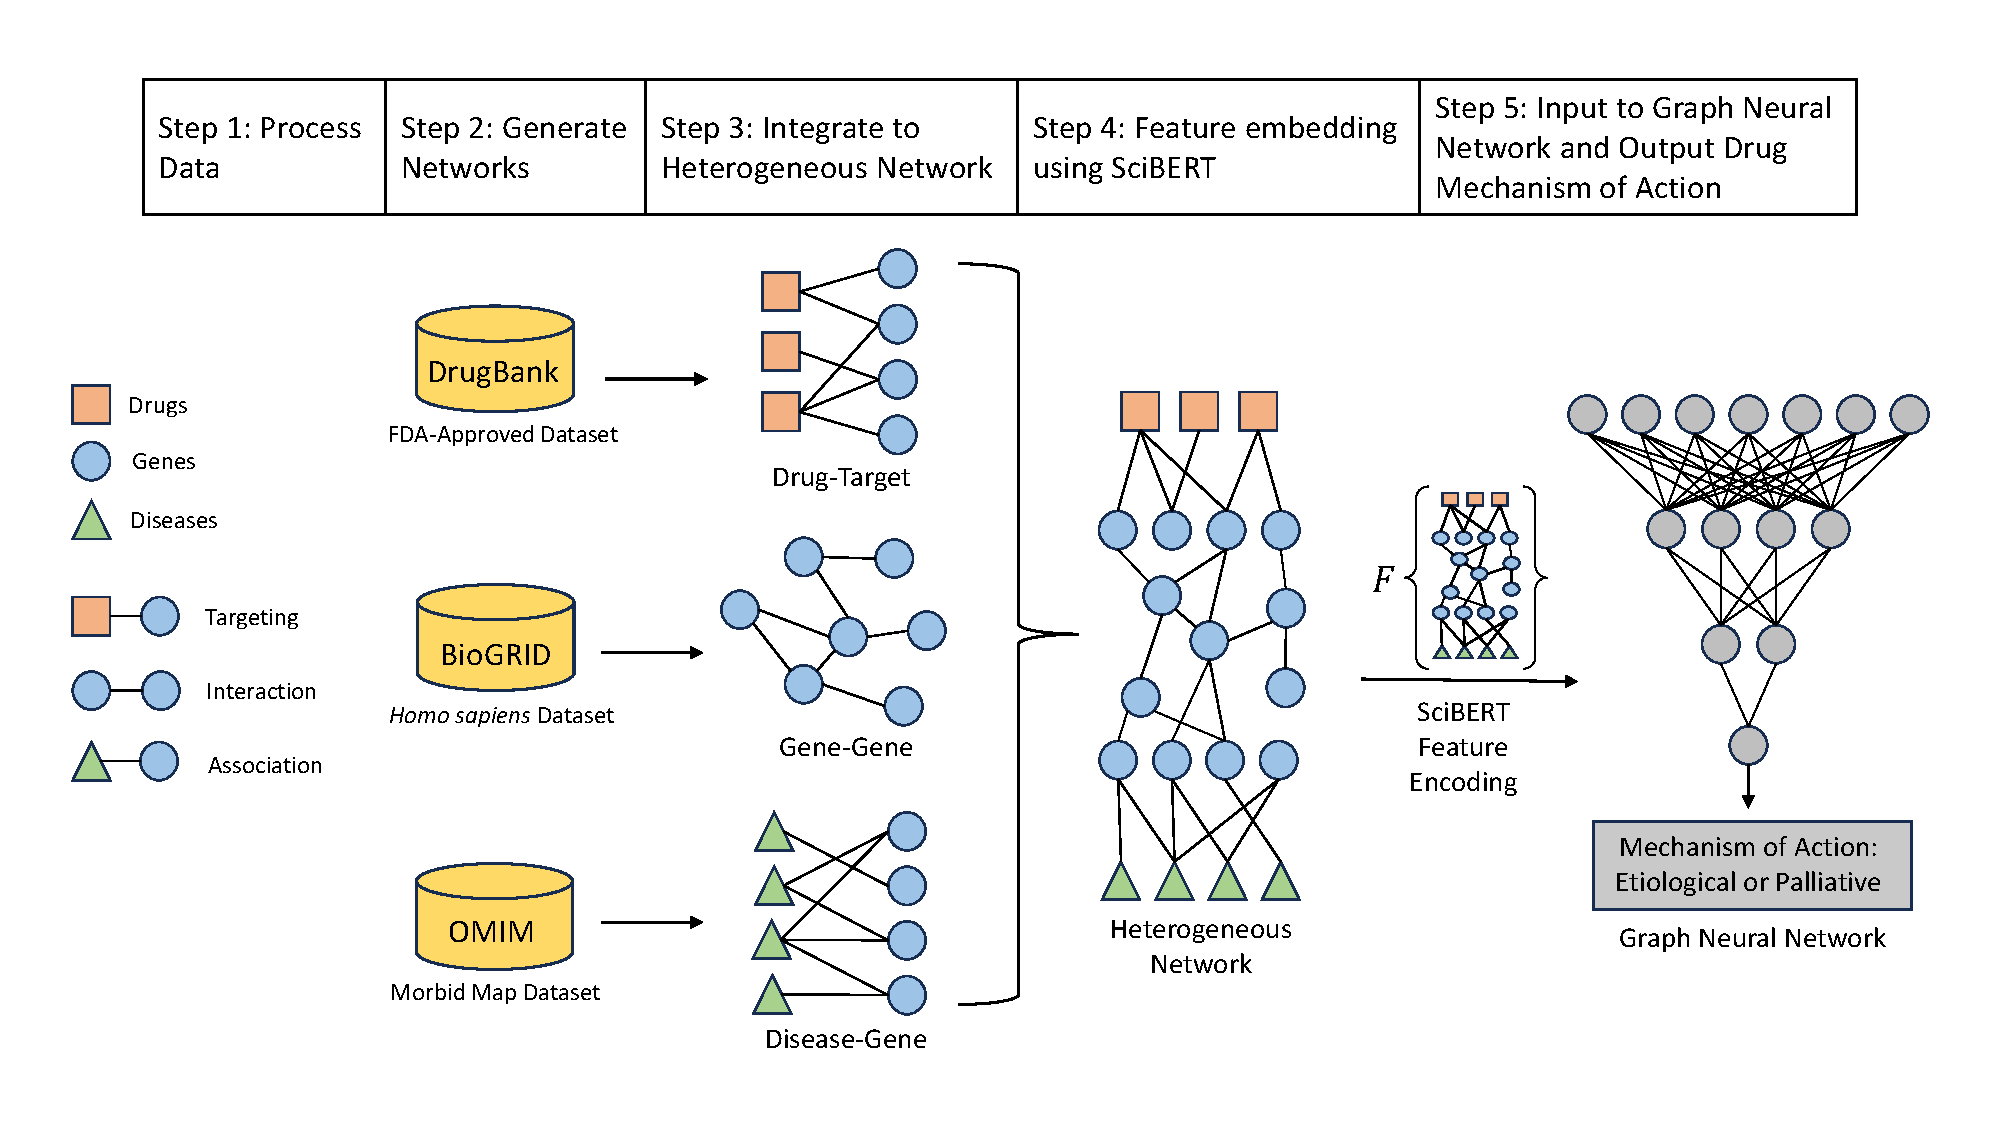
\includegraphics[width=\linewidth]{Figures/FlowChart.pdf}
    \caption{Flowchart of methods employed in this study to build our DruGNNosis-MoA model.
            Illustration of the sequential steps employed to classify drugs as having either etiological or palliative mechanism.
            In Step 1, we acquired and processed our selected datasets, which comprise information on drugs, genes, and diseases.
            In Step 2, we constructed three distinct networks for Drug-Target, Gene-Gene, and Disease-Gene interactions.
            In Step 3, these networks were then integrated to form a comprehensive Heterogeneous network, encompassing a diverse range of node and link (edge) types.
            Following the network integration, in Step 4, we calculated feature embedding on each node type individually utilizing the fine-tuned SciBERT model \cite{beltagy2019scibert}.
            Finally, In Step 5, we streamlined the network embeddings through our Graph Neural Network (GNN) to carry out the classification task, distinguishing each drug node as either etiological or palliative.}
    \label{fig:FlowChart}
\end{figure}

%-----------------------------------------------------------
\section{Results}
\label{sec:res}
%-----------------------------------------------------------
To summarize our analysis steps: We began by manually labeling drugs as etiological and palliative.
Using the labeled set of drugs, we fine-tuned the SciBERT model to classify drugs as etiological or palliative.
Next, we constructed biological networks and trained two GNNs with different configurations.
Finally, we evaluated the performances of the three developed models (two GNNs and fine-tuned SciBERT). We review the results of these analyses in this section.

%-----------------------------------------------------------
\subsection{Drug Mechanism Labeling}
%-----------------------------------------------------------
A residual drug subset (3.816\%, 77) exhibited a dual role of both etiological and palliative mechanisms based on the diseases they address.
This subset was discarded to implement binary classification.
For example, methotrexate acts as a drug with etiological mechanism in cancer treatment by inhibiting cell division, and acts as a drug with palliative mechanism in arthritis treatment by reducing inflammation.
The remaining drugs present a nearly equal distribution of either etiological (47.423\%, 957) or palliative (48.761\%, 984) mechanisms (Supplementary Fig. S1). %\ref{fig:EvsP}).
This differs from \cite{yildirim2007drug}, which reported a prevalence of palliative drugs.
Possible reasons for this difference include the potential changes in drug design trends over 16 years, and the undisclosed classification method \cite{yildirim2007drug}.

%\begin{center}
%[Figure \ref{fig:EvsP} about here.]
%\end{center}

Drugs affiliated to multiple Anatomical Therapeutic Chemical (ATC) classes suggest the possibility of repurposing by utilizing them in different therapeutic categories.
We analyzed how drug mechanisms are distributed across ATC classes (Supplementary Fig. S2)%\ref{fig:EPvsATC})
, inspired by the work of \cite{yildirim2007drug}, who did not directly analyze this distribution \cite[Figure~2]{yildirim2007drug}.
Our analysis revealed distinct distributions within each class.
In the `Nervous System' class, most drugs are palliative (88.484\%, 292), addressing symptoms like pain and psychiatric disorders, but not their underlying causes.
In contrast, drugs in the `Antiinfectives for Systemic Use' class mainly have etiological mechanisms (90.476\%, 57), targeting the root cause of infections such as bacteria and viruses.
Dual-mechanism drugs, addressing both causes and symptoms, make up a small percentage (1.587\% to 7.746\%) across all classes.
This indicates diverse drug roles in different therapeutic areas.

%\begin{center}
%[Figure \ref{fig:EPvsATC} about here.]
%\end{center}

%-----------------------------------------------------------
\subsection{Fine-tuning SciBERT}
%-----------------------------------------------------------
Using drug labeling in the previous section, we fine-tuned the SciBERT model to predict drug labels.
For text inputs into SciBERT, we sourced drug descriptions from DrugBank; gene symbols from BioGRID; and disease names from OMIM.
Following the guidelines of \cite{devlin-etal-2019-bert}, we utilized the Trainer class from Hugging Face \cite{wolf2019huggingface}, with the following parameters:
AdamW optimizer with a weight decay of  $2e^{-3}$:
AdamW differs from standard Adam by its unique approach to weight decay regularization; a learning rate of $2e^{-5}$; a batch size of 16; and a total of 3 training cycles.


SciBERT represented each text as a numeric vector (embeddings vector) of size 768.
Consequently, we obtained three unique matrices of $Entity \times 768$ dimensionality, where Entity (rows) indicate either drugs, genes or diseases; and columns indicate values of the embeddings vectors.
Then, we performed Principal Component Analysis (PCA) to reduce the dimensionality of each matrix to $Entity \times 128$.
The reduced embedding vector for each entity type was integrated into our heterogeneous network as a node (drug, gene, disease) feature.
This integration enhanced the learning capabilities of the GNN in developing more robust and representative node features.

%-----------------------------------------------------------
\subsection{Network Construction}
\label{sec:network_construction_2}
%-----------------------------------------------------------

An overview of the networks analyzed in this project is presented in Table \ref{tbl:networkFeatures}, and descriptions are provided below.

\textbf{Drug-Target Network}
comprises 2,018 drug nodes, 2,232 target-gene nodes, and 10,250 links (edges) connecting them.
It forms 129 connected components, with 75 consisting of standalone drug-target pairs.
We observe a small number of highly connected nodes (hubs) and numerous nodes with only a few connections \cite{barabasi2009scale}.
The Largest Connected Component (LCC) within the network includes 1,797 drug nodes, 2,027 target-gene nodes, and 9,916 links.
Notably, the most frequent degree in the LCC is 1, suggesting a prevalence of nodes with a single connection.
Higher degrees are less frequent, aligning with the hubs that determine the connectivity of the LCC.

\textbf{PPI Network}
comprises 19,893 gene nodes interconnected by 781,272 links, excluding 3,344 self-interactions.
This network has 4 components, with 3 of them consisting of isolated genes.
The most frequent degree is 1, indicating a prevalence of branched-off nodes with a single connection.

\begin{table}
\caption{Summary descriptions of the analyzed networks.
\label{tbl:networkFeatures}}%
\begin{threeparttable}
\begin{tabular*}{\columnwidth}{@{\extracolsep\fill}llll@{\extracolsep\fill}}
\toprule
Network & \# Nodes  & \# Links (Edges)\\
\midrule
Drug-Target               & 2,018 drugs    & 10,250\\
                          & 2,232 genes            \\
\midrule
PPI                       & 19,893 genes   & 781,272\\
\midrule
Disease-Gene              & 8,156 diseases & 27,692\\
                          & 16,358 genes           \\  
\midrule
Heterogeneous\tnote{*}    & 1,941 drugs   & 822,086\\
                          & 31,524 genes           \\
                          & 8,156 diseases         \\
\bottomrule
\end{tabular*}
\begin{tablenotes}
\item[*] The heterogeneous network's topological features were calculated while excluding drugs labeled as 'both'.
\end{tablenotes}
\end{threeparttable}
\end{table}




\textbf{Disease-Gene Network}
comprises 8,156 disease nodes, 16,358 associated-gene nodes, and 27,692 links (edges) connecting them.
This network is organized into 5,430 connected components, with 1,065 being standalone disease-gene pairs.
Each component features a unique set of diseases and genes that are closely interconnected.
Within this network, the LCC consists of 265 disease nodes, 379 associated-gene nodes, and 1,493 links (edges).
The most frequent degree in the LCC is 2, indicating that the majority of diseases or genes in this component are connected to two other genes or diseases.


\textbf{Heterogeneous Network}
comprised of 1,941 drug nodes (excluding those displaying both etiological and palliative mechanisms), 31,524 gene nodes, and 8,156 disease nodes.
The link types include 9,778 drug-gene links, 784,616 gene-gene links, and 27,692 disease-gene links, for a total of 822,086 edges.

For each of the two developed GNN models, we computed the following node feature matrices: (i) EigenVector features for the Baseline GNN model; and
(ii) textual features (embeddings of the fine-tuned SciBERT model) for the developed DruGNNosis-MoA model.
In both models, drug nodes are assigned a label of either etiological or palliative.


% Network analysis
%The network analysis revealed a distinct pattern characterized by an abundance of nodes with sparse connections and a minority of heavily interconnected nodes.
%The distribution of node degrees follows a power-law curve, a characteristic feature of scale-free networks found in various real-world systems \cite{broido2019scale,barabasi2009scale}.
%These networks exhibit highly connected nodes (hubs), resilience to random failures, efficient information flow, emergent behaviors, and heterogeneity in connectivity \cite{broido2019scale}.
%Logarithmic transformation confirmed an alignment between the link distribution of nodes and the curve, resembling distributions observed in real-world scenarios \cite{barabasi2009scale,clauset2009power,fortunato2006scale}.
%Statistical analysis methods yielded a p-value of 0.00004, providing additional support for the presence of a scale-free distribution.

Topological analyses revealed a significant occurrence of ``follow-on" drugs.
These are drugs that target proteins that have already been selected targets for previous drugs.
This trend reflects a prevailing strategy within the pharmaceutical industry to concentrate efforts on well-established target proteins, resulting in an accumulation of such drugs that target proteins already targeted by existing drugs \cite{aronson2020me}.
This strategy limits drug discovery to a narrow range of target proteins, restricting the exploration of novel targets

Fig. \ref{fig:heteroSubGraph} illustrates a sub-graph of our heterogeneous network exhibiting the occurrence of follow-on drugs linked to colorectal cancer (green) genes.
Within this sub-graph, there are a total of 48 genes (blue) associated with colorectal cancer, with some connections to other genes.
A smaller subset of these genes is targeted by drugs (orange), revealing a clustering effect of drugs focused on specific targets.
Notably, the majority of these drugs are categorized as having etiological mechanisms, aligning with our findings that most drugs designed to combat cancer primarily work by inhibiting cell division and hindering growth.
Our GNN models utilize this heterogeneous network for learning how to classify drugs as having either etiological or palliative mechanism, explained next.

%\begin{center}
%[Figure \ref{fig:heteroSubGraph} about here.]
%\end{center}
\vspace{-2em}
\begin{figure}[H]
    \centering
    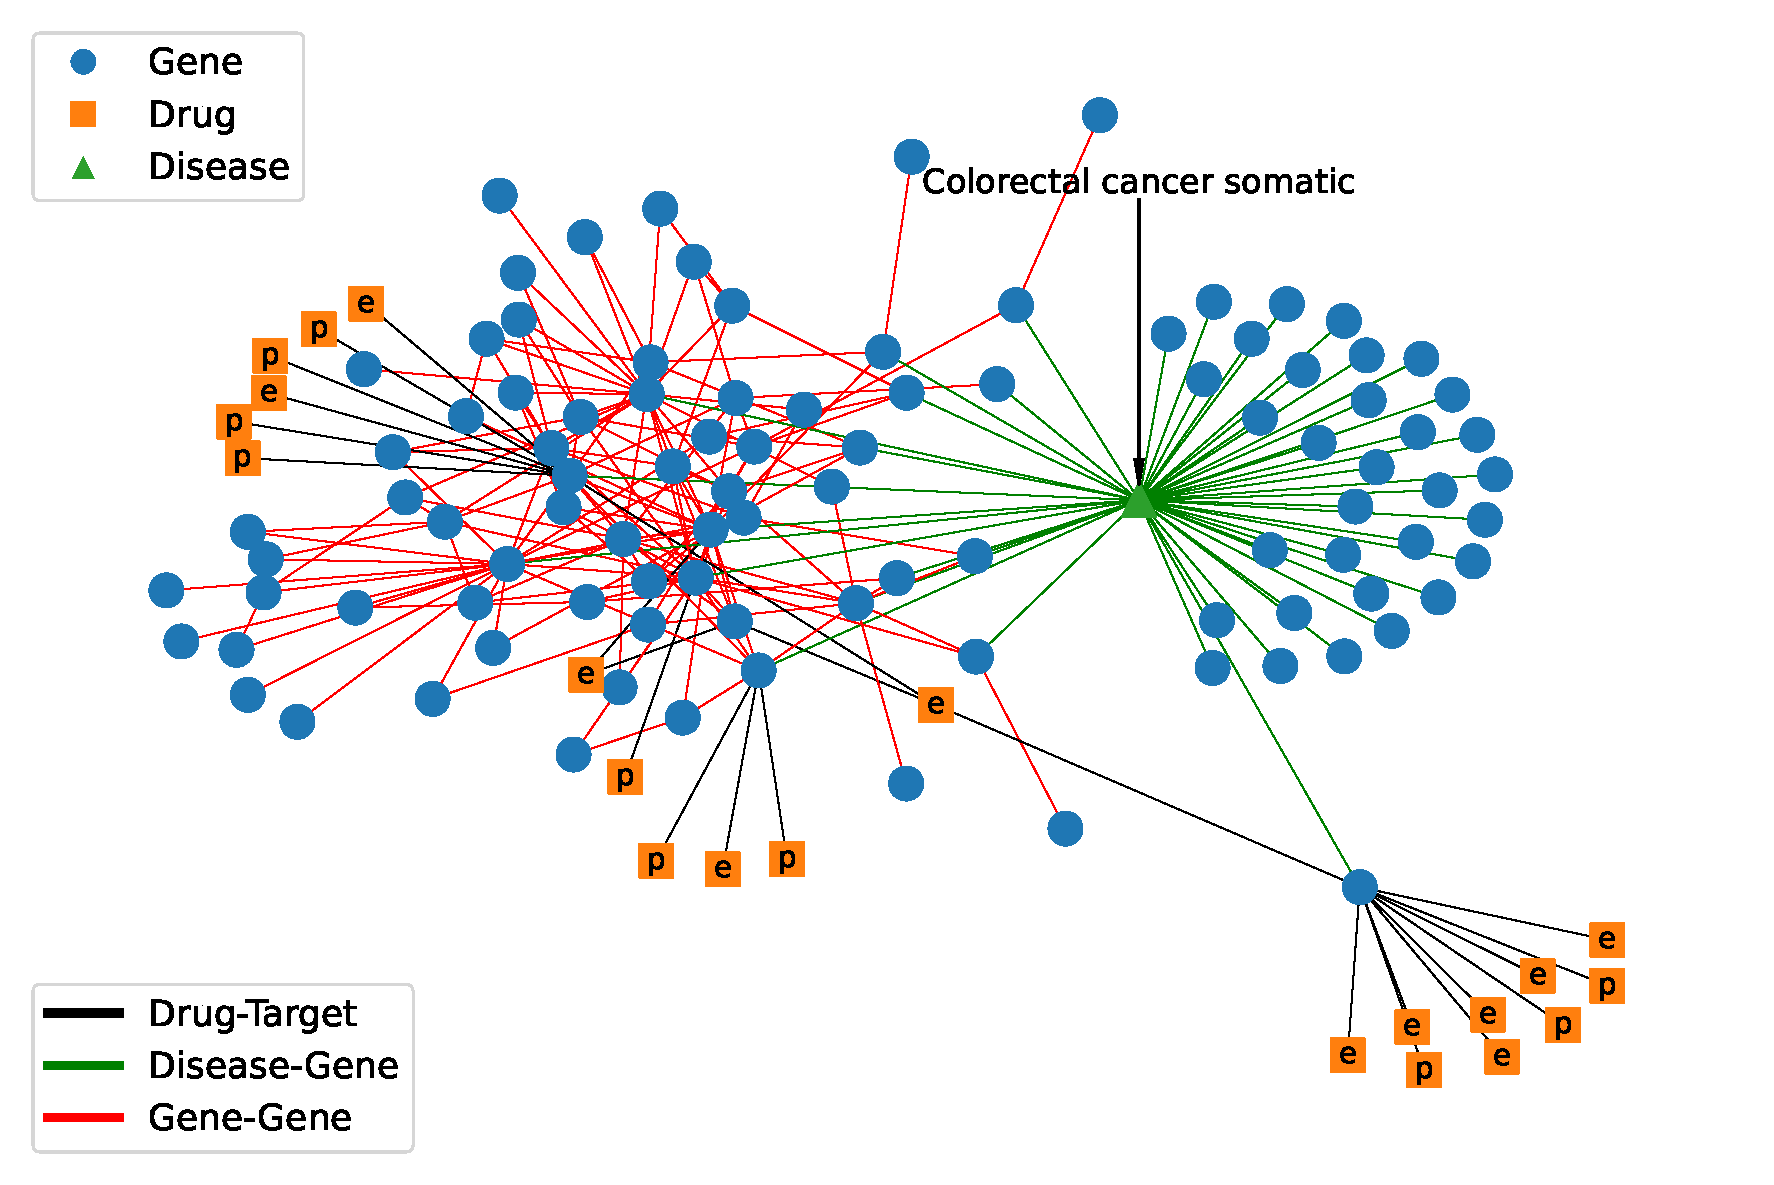
\includegraphics[width=\linewidth]{Figures/heterogeneous_networks.pdf}
    \caption{ \text{Example sub-graph of our heterogeneous network}. The disease colorectal cancer (green triangle) is connected directly and indirectly to numerous genes (blue dots).
    For visualization purposes, we selected all directly linked genes, and some indirectly linked genes, to sum to 50 in total.
    Some of these genes are targeted by drugs (orange squares). Each drug is labeled as having etiological (`e') or palliative (`p') mechanism.
    ``Follow-on" drugs, which are drugs targeting the same gene as other drugs, can be seen.
    This network shows the existence of many potential gene targets for colorectal cancer, yet only a few have been selected for drug treatment, to date. Additionally, this sub-graph reveals a dominance of etiological drugs, correlating with our findings of the `L’ ATC class.}
    \label{fig:heteroSubGraph}
\end{figure}


%-----------------------------------------------------------
\subsection{Graph Neural Network Training}
%-----------------------------------------------------------
In terms of model architecture, both the Baseline GNN and the DruGNNosis-MoA models developed in this study share several components.
These include two SageConv layers, the ReLU activation function, the Adam optimizer with learning rates of $5e^{-4}$ for the Baseline GNN model and  $6e^{-4}$ for the DruGNNosis-MoA model, a sigmoid function on the output, and a gradient clipping technique with a threshold set at 0.5 to prevent gradient explosion and ensure stable, efficient training.
However, for the DruGNNosis-MoA model, this approach proved insufficient for preventing overfitting, leading to the incorporation of an additional dropout strategy after the first layer, set at a probability of 0.3.
Dropout works by randomly deactivating a portion of nodes during training, which helps to reduce overfitting by preventing complex co-adaptations on training data.
The primary distinction between training the two models lay in the number of epochs required to achieve the optimal solution.
The DruGNNosis-MoA model needed just 30 epochs, while the Baseline GNN model required 100 epochs.
Moreover, node features play a key role in GNN training, significantly affecting the model's performance and behavior. %\cite{mahmoud2023node, duong2019node}.
A major difference between the two developed models lies in their node features: the Baseline GNN model uses features derived from EigenVector matrices, whereas the DruGNNosis-MoA uses features extracted from text.

%-----------------------------------------------------------
\subsection{Model Evaluation}
%-----------------------------------------------------------
To compare the 3 developed models (fine-tuned SciBERT, Baseline GNN, and DruGNNosis-MoA), we used a 10-fold cross-validation (CV) process.
For each fold, we computed the accuracy score, F1-scores, precision, recall, and ROC-AUC score (Area Under the Curve).
Then, we calculated the average score and standard deviation for each matrix (Table \ref{tbl:cv_scores}).

\begin{table}
\caption{Cross-validation metric scores of different models.
\label{tbl:cv_scores}}%
\begin{tabular*}{\columnwidth}{@{\extracolsep\fill}lllll@{\extracolsep\fill}}
\toprule
Model & Metrics & Average & S.D \\
\midrule
Baseline GNN & Accuracy    & 0.699   & 0.034 \\
             & F1-score         & 0.664   & 0.043 \\
             & Precision         & 0.715   & 0.051 \\
             & Recall            & 0.622    & 0.045 \\
             & ROC-AUC     & 0.787   & 0.03 \\
\midrule
Fine-Tuned SciBERT & Accuracy    & 0.906   & 0.018 \\
                   & F1-score         & 0.906   & 0.018 \\
                   & Precision         & 0.895   & 0.028 \\
                   & Recall            & 0.918   & 0.012 \\
                   & ROC-AUC     & 0.961   & 0.012 \\
\midrule
DruGNNosis-MoA & Accuracy    & 0.938    & 0.017 \\
            & F1-score         & 0.935   & 0.017 \\
            & Precision         & 0.931   & 0.029 \\
            & Recall            & 0.941   & 0.022 \\
            & ROC-AUC     & 0.977   & 0.001 \\
\bottomrule
\end{tabular*}
\begin{tablenotes}%
\item[*] S.D. - Standard deviation
\end{tablenotes}
\end{table}


Initially, we evaluated the F1-score performance across the 10-fold CV by generating comparative plots for the three models (Fig. S3a).%\ref{fig:fscore1a}.
We then closely examined the performance trends of the two top models, fine-tuned SciBERT and DruGNNosis-MoA (Fig. S3b).% \ref{fig:fscore1b})

The DruGNNosis-MoA model shows higher F1-scores in every fold when compared with the SciBERT model, with the exception of folds 1 and 8, where their performance converges.
Notably, in about half of the folds, the DruGNNosis-MoA model achieves excellent F1-score performance, reaching as high as 0.955.
This pattern suggests a trend where DruGNNosis-MoA outperforms SciBERT in the task of classifying drugs as etiological or palliative (Fig. S3b). %\ref{fig:fscore1b}).

% The following information is from before we changed the code, and is being retained for reference in future changes: (Unfortunately, following the code modifications, the std of both SciBERT and DruGNNosis-MoA models are now nearly identical. SciBERT have std of 0.014, while DruGNNosis-MoA have higher std of 0.016.)
% This figure also indicates that the performance of DruGNNosis-MoA is consistent, with less variation in F1 scores between folds.
% In contrast, SciBERT exhibits more variation in scores, with certain folds showing notably lower F1 scores.
% The average F1 score achieved by DruGNNosis-MoA is 0.94, with a standard deviation of 0.0049, compared with SciBERT, which has an average F1 score of 0.9, with a standard deviation of 0.0084.

%--------------------------------
%\subsection{DruGNNosis-MoA Performance}
%--------------------------------
% After observing that the DruGNNosis-MoA model demonstrated superior performance in classifying drugs on unseen data, consistently outperforming in each fold and exhibiting overall excellence, along with the highest stability (lowest standard deviation), we assessed its efficacy through the ROC-AUC curve.

After observing that the DruGNNosis-MoA model demonstrated superior performance for F1-score, we assessed its efficacy via the ROC-AUC curve.
We compare the three models using the average ROC-AUC curves (Fig. S4).%\ref{fig:roc_auc1}).


%\begin{center}
%[Figure \ref{fig:roc_auc1} about here.]
%\end{center}

% The ROC-AUC curve, as shown in Figure \ref{fig:roc_auc1}, demonstrates consistency in the model's performance, with most folds achieving an Area Under the Curve (AUC) nearly reaching 0.98.
%In the ROC-AUC, our focus is on comparing the average scores across models rather than individual model performance like we did before the changes.

The ROC-AUC curve, as shown in Fig. S4,
%\ref{fig:roc_auc1}, 
demonstrates the DruGNNosis-MoA model's consistently superior performance in classifying drugs.
It achieves an impressive average Area Under the Curve (AUC) of 0.977, complemented by the highest level of stability, indicated by the lowest standard deviation of 0.001.
These results indicate a difference in performance between the DruGNNosis-MoA model and the fine-tuned SciBERT model, with implications for their respective efficacy in drug classification tasks.

Overall, we observe that our DruGNNosis-MoA model outperformed all other models in terms of the average Accuracy Score, F1-score, Precision, Recall, and ROC-AUC Score (Table \ref{tbl:cv_scores}).
In the evaluation of the DruGNNosis-MoA model, the highest standard deviation (S.D.) observed was 0.029 in the precision metric, while the lowest S.D., 0.001, was found in the ROC-AUC metric.
Notably, this ROC-AUC S.D. is the smallest across all matrices and models.

Therefore, we selected and applied the DruGNNosis-MoA model to our Test set,
resulting in an F1-score of 0.942 and a ROC-AUC value of 0.975.
These results further reinforce the consistent superiority of the DruGNNosis-MoA model in drug classification performance on previously unseen data.

%--------------------------------
\section{Discussion and Conclusions}
%--------------------------------
Elucidating drug mechanisms as etiological or palliative is crucial for drug design and treatment selection. 
Understanding these mechanisms can guide the development of new drugs and the repurposing of existing ones. 
Our findings show a balance between etiological and palliative mechanisms among FDA-approved drugs.

While the topic has been widely studied, systematic classification using modern computational methods remains underexplored. 
Our work extends beyond previous network-based analyses by incorporating Graph Neural Networks (GNNs) and Large Language Models (LLMs), revealing novel associations not previously identified.

The distinction between etiological and palliative mechanisms prompts a consideration of whether a drug aims to address root causes or alleviate symptoms. 
This differentiation is vital for advancing medical treatments.

Our DruGNNosis-MoA model outperformed other models, including the fine-tuned SciBERT model, by using text input to enhance performance. 
The combination of GNN and SciBERT in DruGNNosis-MoA proved superior, particularly in generalizing to unseen data.

Our novel DruGNNosis-MoA model integrates diverse data, uncovering hidden relationships in drug-gene-disease interactions. 
This study is pioneering in using a language-network framework with machine learning to explore these mechanisms, offering insights beyond conventional distance-based methods.

Contrasting with prior studies, our findings suggest a shift towards targeting root causes or a difference due to methodological changes. Unlike distance-based approaches, our analysis found no significant correlation between a drug's mechanism of action (MoA) and the distance from disease genes.

Examining individual ATC classes revealed that the balance of etiological and palliative mechanisms does not apply universally.
We also identified drugs with dual mechanisms, challenging the binary classification and highlighting the complexity of drug actions.

%--------------------------------
%\section{Conclusions}
%--------------------------------
Our method's limitations include potential subjectivity in labeling mechanisms as etiological or palliative, based on DrugBank data.
Some drugs have multiple conditions listed, complicating the classification. 
Future work should refine these labels and explore specific drug mechanisms in detail.

We acknowledge that labeling a drug as etiological doesn't imply a cure, as some data include diseases not officially approved for treatment.
Expanding features, such as chemical structures, could improve model performance.

Our study offers avenues for further research, including exploring novel drug targets, analyzing success rates by drug mechanism, and focusing on specific ATC classes for a deeper understanding of relationships within the network.

The approach presented advances the systematic assessment of drug mechanisms using cutting-edge computational methods, enhancing precision and efficiency in drug development.


%\section{Competing interests}
%The authors declare no competing interests.

%\section{Author contributions statement}
%L.B. contributed Investigation, Formal Analysis, Methodology, Software, Validation, Visualization, Writing – original draft, and Writing - review and editing. 
%E.B. contributed Investigation, Formal Analysis, Data curation, Validation, Visualization, Writing – original draft, and Writing - review and editing. 
%K.M.J. contributed Conceptualization, Data curation, Funding acquisition, Methodology, Project administration, Supervision, Validation, Visualization, Writing – original draft, and Writing – review and editing. 
%A.B. contributed Conceptualization, Formal analysis, Funding acquisition, Investigation, Methodology, Project administration, Resources, Software, Supervision, Visualization, Writing – original draft, and Writing – review and editing.

%\section{Acknowledgments} 
%This work is supported in part by funds from Bar-Ilan University's Data Science Institute (DSI). K.M.J. was funded by a Postdoctoral Fellowship from the Mortimer B. Zuckerman STEM Leadership Program.


%square brackets. 
%Multiple references are each numbered with separate brackets. 
%---------------------------------------------------------------------
\section*{Acknowledgment}
%---------------------------------------------------------------------


%---------------------------------------------------------------------
\bibliographystyle{IEEEtran} % or ieeetr, plain, etc.
\bibliography{References}
%---------------------------------------------------------------------


\newpage
%---------------------------------------------------------------------
\appendices
%---------------------------------------------------------------------
%\begin{appendices}

\setcounter{figure}{0}
\renewcommand\thefigure{S\arabic{figure}} % Redefine table numbering style

\twocolumn[\section*{Supplementary material for: DruGNNosis-MoA: Elucidating Drug Mechanisms as Etiological or Palliative With Graph Neural Networks Employing a Large Language Model}]
%-------------------
\section{Supplementary Tables}
\label{sec11}
%-------------------
\subsection{Supplementary Table S1}
Tab 1 of the Supplementary Table S1 contains the supplementary materials related to the drug mechanism annotations and can be accessed through the GitHub repository located at: \url{https://github.com/bartala/PalliativEtiological/tree/main/Supplementary}.

%-------------------
%\subsection{Supplementary Table S2}
%-------------------
Tab 2 of the Supplementary Table S1 contains the supplementary materials related to the example drug mechanism and can be accessed through the GitHub repository located at \url{https://github.com/bartala/PalliativEtiological/tree/main/Supplementary}.

%-------------------
\section{Supplementary Figures}
%-------------------
\begin{figure}[H]
    \centering
    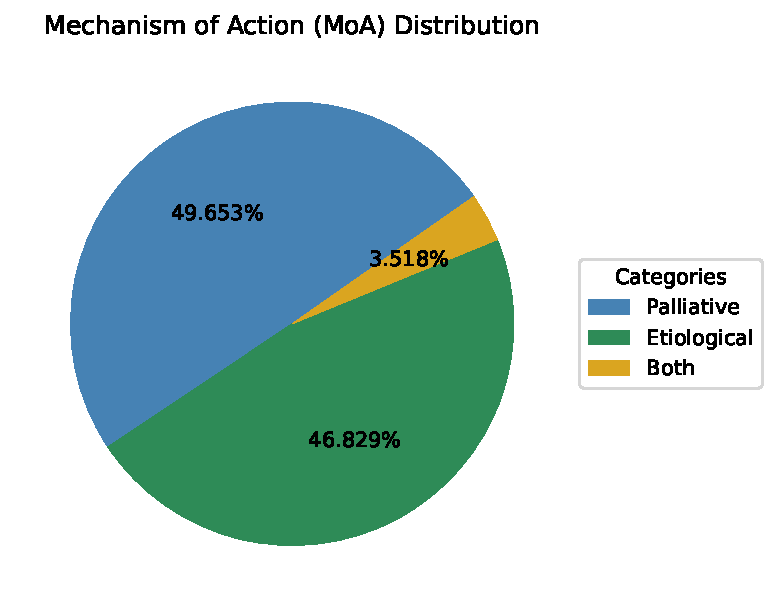
\includegraphics[width=\linewidth]{Figures/EvsP.pdf}
    \caption{Distribution of drug mechanisms of action. The number of etiological and palliative drugs is well balanced, with 47.423\% (957) being etiological, and 48.761\% (984) being palliative.
    Only a small percentage (3.816\%, 77) of drugs exhibit both mechanisms.}
    \label{fig:EvsP}
\end{figure}


%-------------------
%\section{Supplementary Fig. D: Distribution of drug mechanisms across Anatomical Therapeutic Chemical (ATC) classes}
%-------------------
\begin{figure}[H]
    \centering
    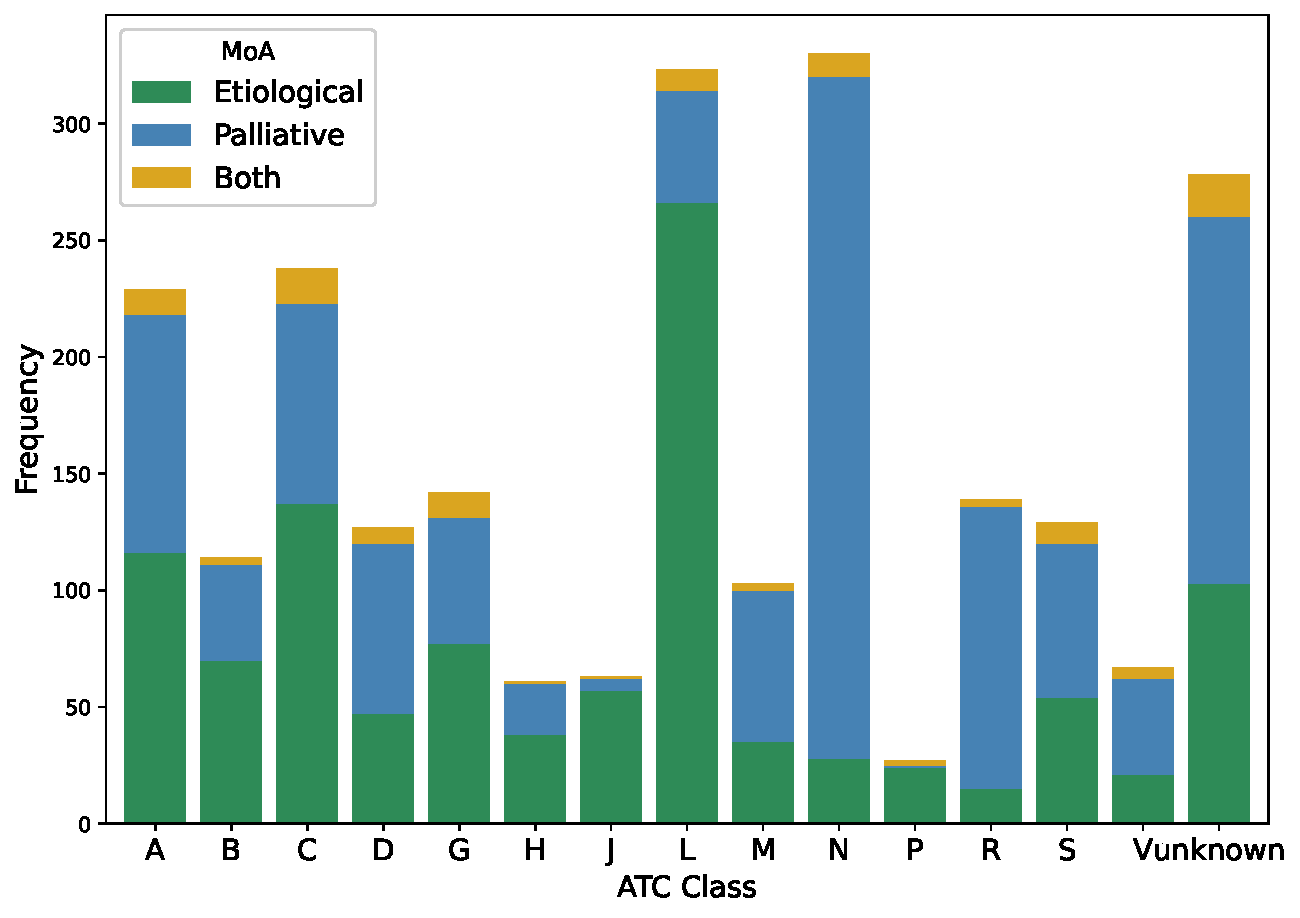
\includegraphics[width=\linewidth]{Figures/EPvsATC.pdf}
    \caption{ Distribution of drug mechanisms across Anatomical Therapeutic Chemical (ATC) classes.
    Each ATC class has a unique distribution of drug mechanisms.
    Some classes, e.g., `J', `L', and `P', are mainly associated with drugs having etiological mechanisms.
    In contrast, classes like 'N' and `R' are primarily associated with drugs having palliative mechanisms.
    The remaining classes generally exhibit a balance between drugs with etiological and palliative mechanisms.
    ATC Class Definitions:
   ``A": Alimentary tract and metabolism;
   ``B": Blood and blood forming organs;
   ``C": Cardiovascular system;
   ``D": Dermatologicals;
   ``G": Genito urinary system and sex hormones;
   ``H": Systemic hormonal preparations, excluding sex hormones and insulins;
   ``J": Antiinfectives for systemic use;
   ``L": Antineoplastic and immunomodulating agents;
   ``M": Musculo-skeletal system;
   ``N": Nervous system;
   ``P": Antiparasitic products, insecticides and repellents;
   ``R": Respiratory system;
   ``S": Sensory organs;
   ``V": Various;
   "Unknown": Drug entries that do not have an ATC class assigned to them in DrugBank.
    }
    \label{fig:EPvsATC}
\end{figure}


%-------------------
%\section{Supplementary Fig. E: Comprehensive overview of the F1-score performance of three models developed in this study to classify drugs as having etiological or palliative mechanism}
%-------------------

\begin{figure}[H]
\centering
\begin{subfigure}[H]{\linewidth}
   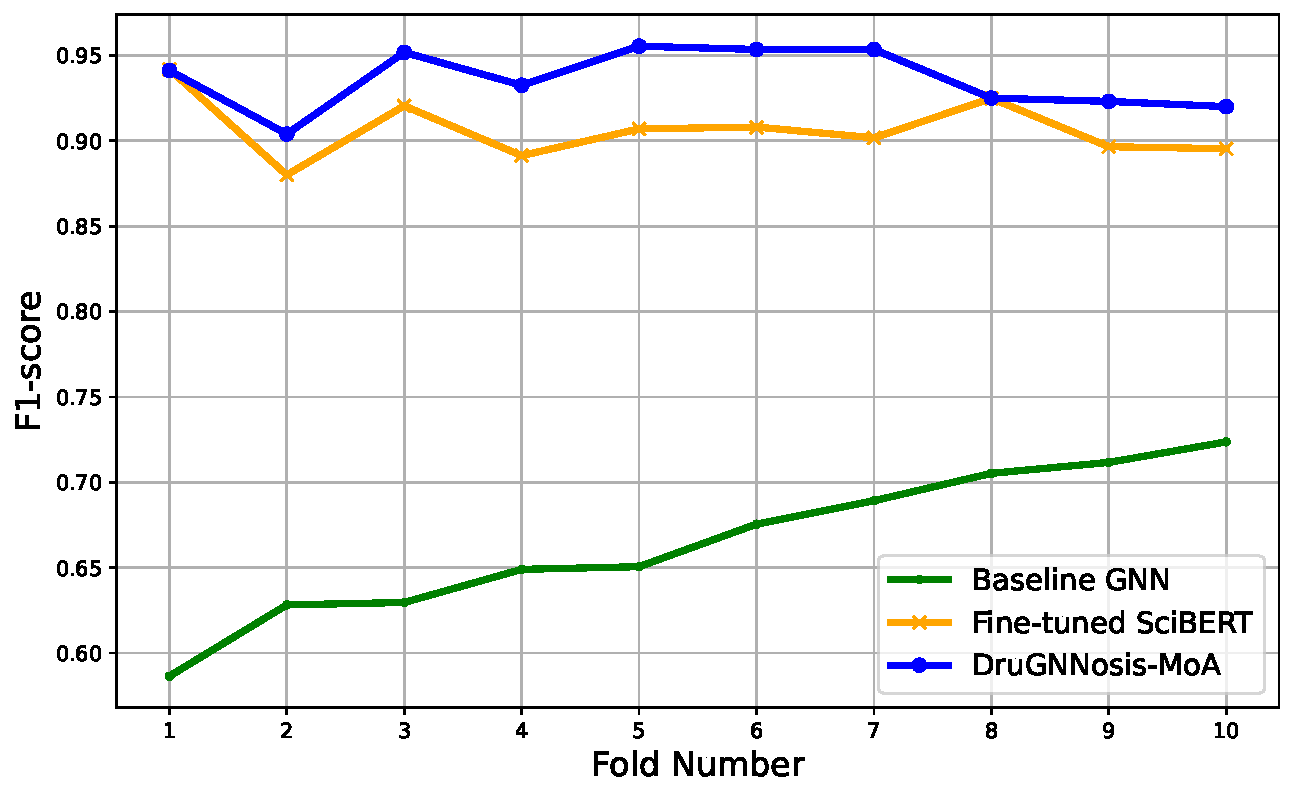
\includegraphics[width=\linewidth]{Figures/Comparison_F1_Scores_3_models.pdf}
   \caption{Comprehensive overview of the F1-score performance of three models developed in this study to classify drugs as having etiological or palliative mechanism.
   The results of the Baseline GNN model are characterized by an average F1-score of 0.664 and standard deviation of 0.043.
   Among the three models, the Baseline GNN model exhibits the lowest performance.
   The blue line represents our DruGNNosis-MoA model, the orange line represents the SciBERT model \citep{beltagy2019scibert}, and the green line represents the Baseline GNN model.}
   \label{fig:fscore1a}
\end{subfigure}
\begin{subfigure}[H]{\linewidth}
   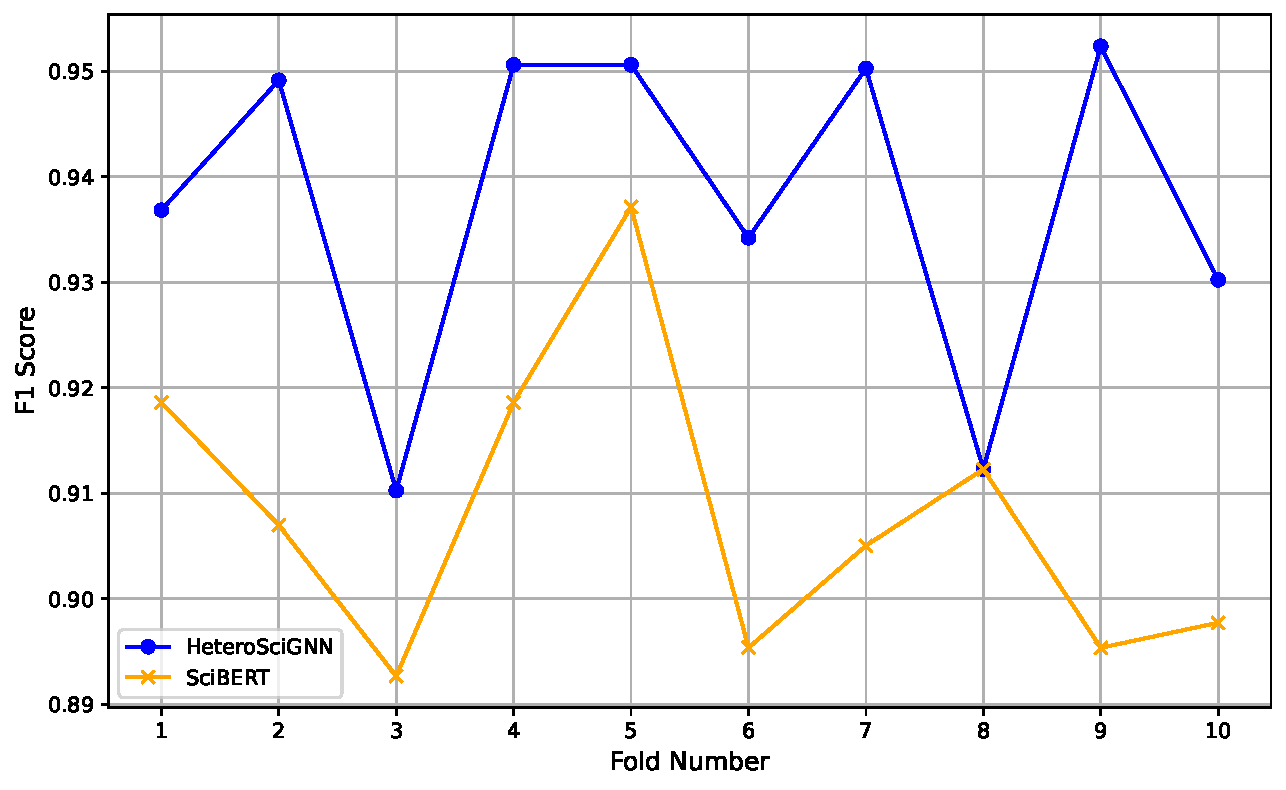
\includegraphics[width=\linewidth]{Figures/Comparison_F1_Scores_2_models.pdf}
   \caption{Comparison of F1-scores between the DruGNNosis-MoA and SciBERT models.
   Each point on the lines corresponds to the F1-score obtained for that particular fold of the cross-validation.
   There is a clear observation that the DruGNNosis-MoA model performed better on a fold-by-fold basis.}
   \label{fig:fscore1b}
\end{subfigure}
\caption{F1-score comparisons for different models.}
\label{fig:fscore1}
\end{figure}



%-------------------
%\section{Supplementary Fig. F: Receiver operating characteristic (ROC) curve of three models to classify drugs as having etiological or palliative mechanism}
%-------------------

\begin{figure}[H]
\centering
\begin{subfigure}[H]{\linewidth}
   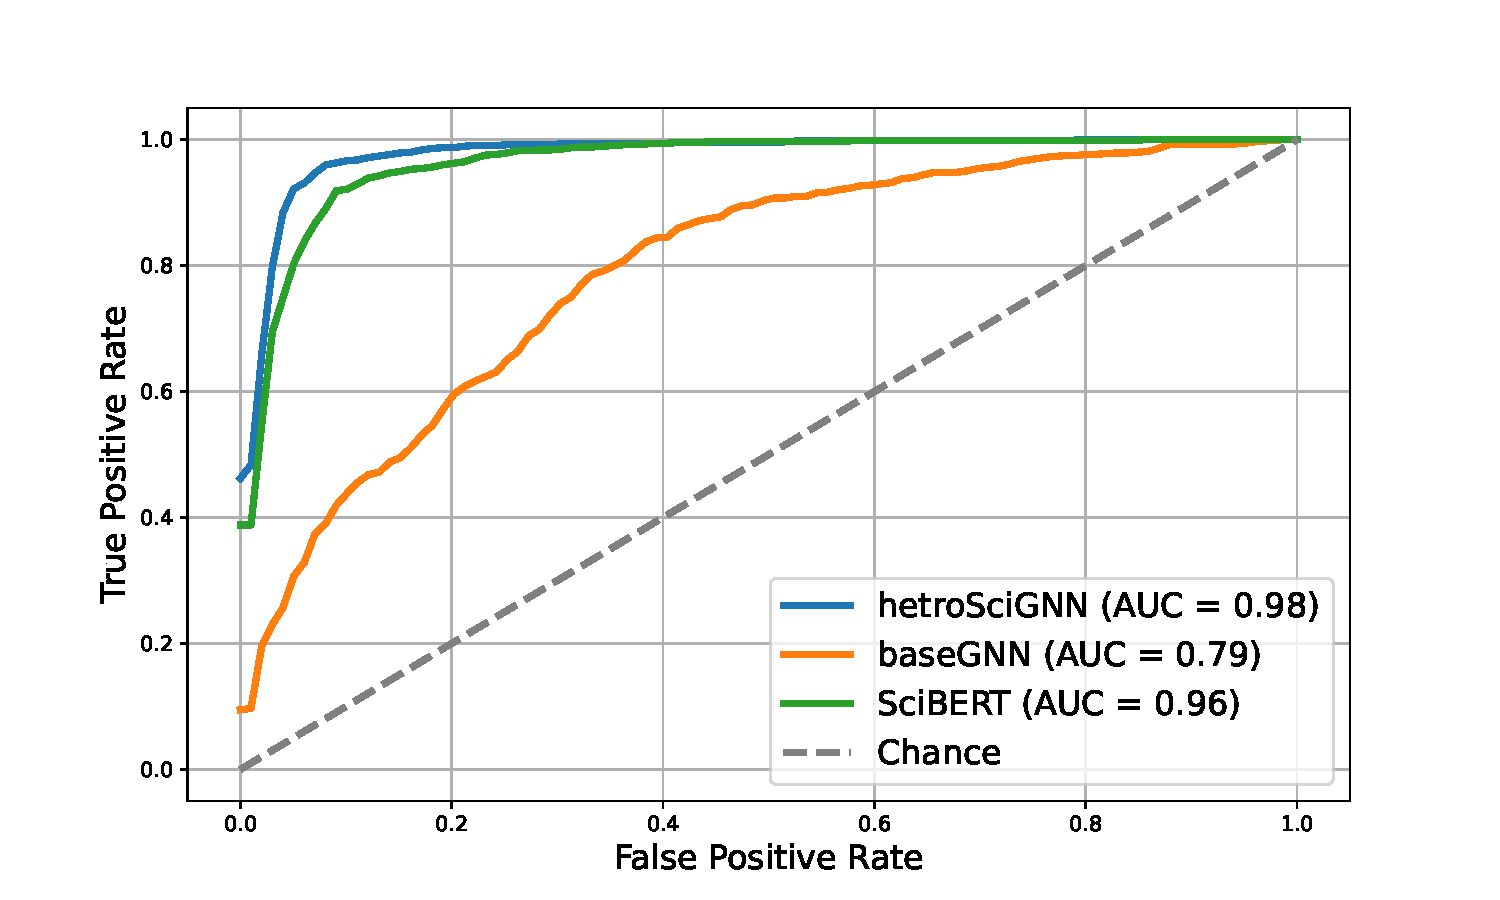
\includegraphics[width=\linewidth]{Figures/3_Models_Roc.pdf}
   \caption{
    Receiver operating characteristic (ROC) curve of three models to classify drugs as having etiological or palliative mechanism.
    The ROC curve compares the performance of three models over 10-fold cross-validation: Baseline GNN (blue), Fine-tuned SciBERT (orange), and DruGNNosis-MoA (green).
    Each line denotes the average ROC- Area Under Curve (AUC) for a model, indicating its True Positive Rate against the False Positive Rate.
    The dashed line represents the performance of a random (by chance) classifier, for reference.}
   \label{fig:roc_auc1a}
\end{subfigure}
\begin{subfigure}[H]{\linewidth}
   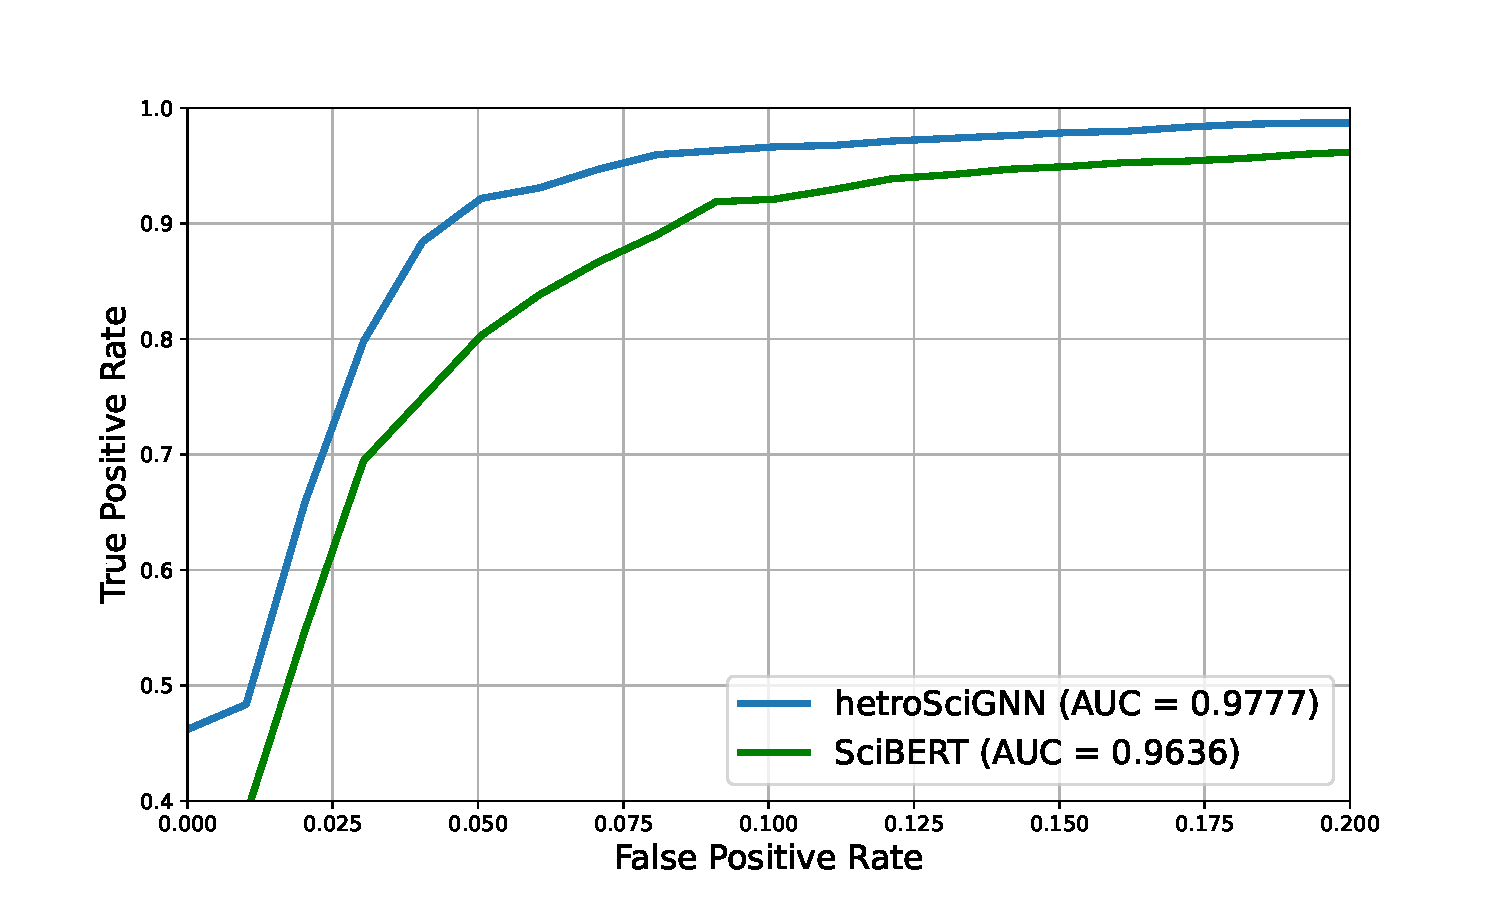
\includegraphics[width=\linewidth]{Figures/LLM_GNN_ROC_AUC.pdf}
   \caption{
    ROC curve highlighting the performance of the two top-performing models over 10-fold cross-validation: Fine-tuned SciBERT model (orange) and our DruGNNosis-MoA model (blue).
    Each line represents the average 10-fold CV ROC-AUC for a model, indicating its True Positive Rate (ranging from 0.4 to 1) against the False Positive Rate (ranging from 0 to 0.2).}
   \label{fig:roc_auc1b}
\end{subfigure}
\caption{Receiver Operating Characteristic (ROC) curves comparing the performance of three models to classify drugs as having etiological or palliative mechanism.}
\label{fig:roc_auc1}
\end{figure}



%-------------------
%\section{Supplementary Fig. G: All vs. All (Comprehensive) Method} 
%-------------------

\begin{figure}[H]
\centering
\begin{subfigure}[H]{\linewidth}
   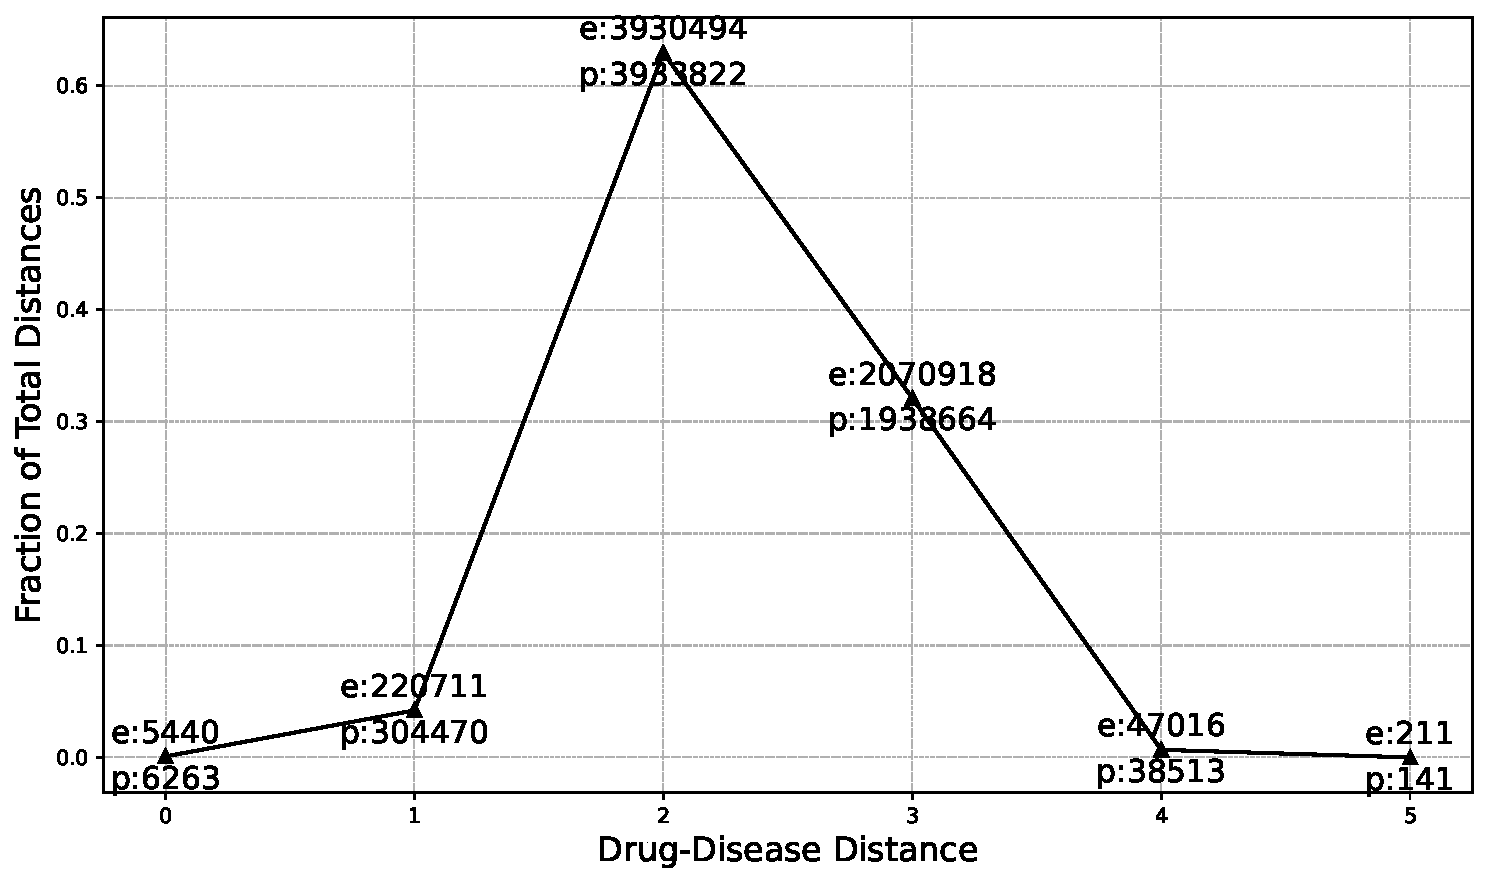
\includegraphics[width=\linewidth]{Figures/Yildrim_all_shortest_distance.pdf}
   \caption{\textbf{All vs. All (Comprehensive) Method:} Calculates and counts the shortest distance between each drug and disease pair, considering each occurrence of the drug in multiple paths.
   According to the technique of \cite{yildirim2007drug}, distances 0 and 1 hold statistical significance and are considered to indicate etiological drug mechanisms.}
   \label{fig:yildirim1}
\end{subfigure}
\begin{subfigure}[H]{\linewidth}
   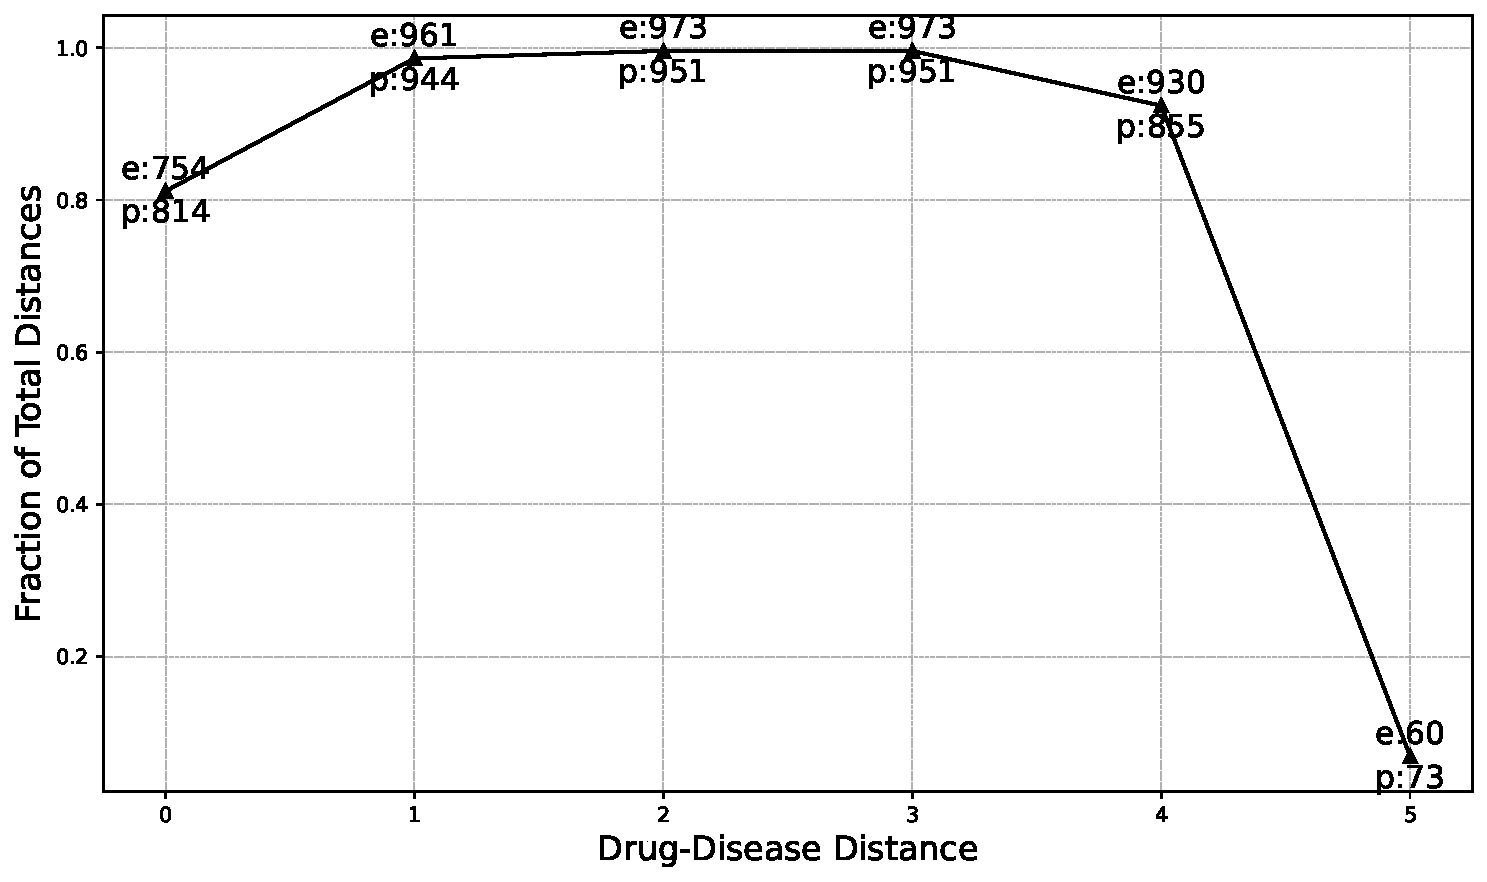
\includegraphics[width=\linewidth]{Figures/Yildrim_ALL_unique_drug_count_shortest_distance.pdf}
   \caption{\textbf{All vs. All (Unique) Method:} 
   Calculates the shortest distances between each drug and disease pair using a distinct counting mechanism. A drug is counted only once at each unique distance, regardless of how many times it appears at that distance. This ensures a balanced representation of drug applications relative to distance, preventing overemphasis on drugs appearing multiple times at the same distance.}
   \label{fig:yildirim2}
\end{subfigure}
\begin{subfigure}[H]{\linewidth}
   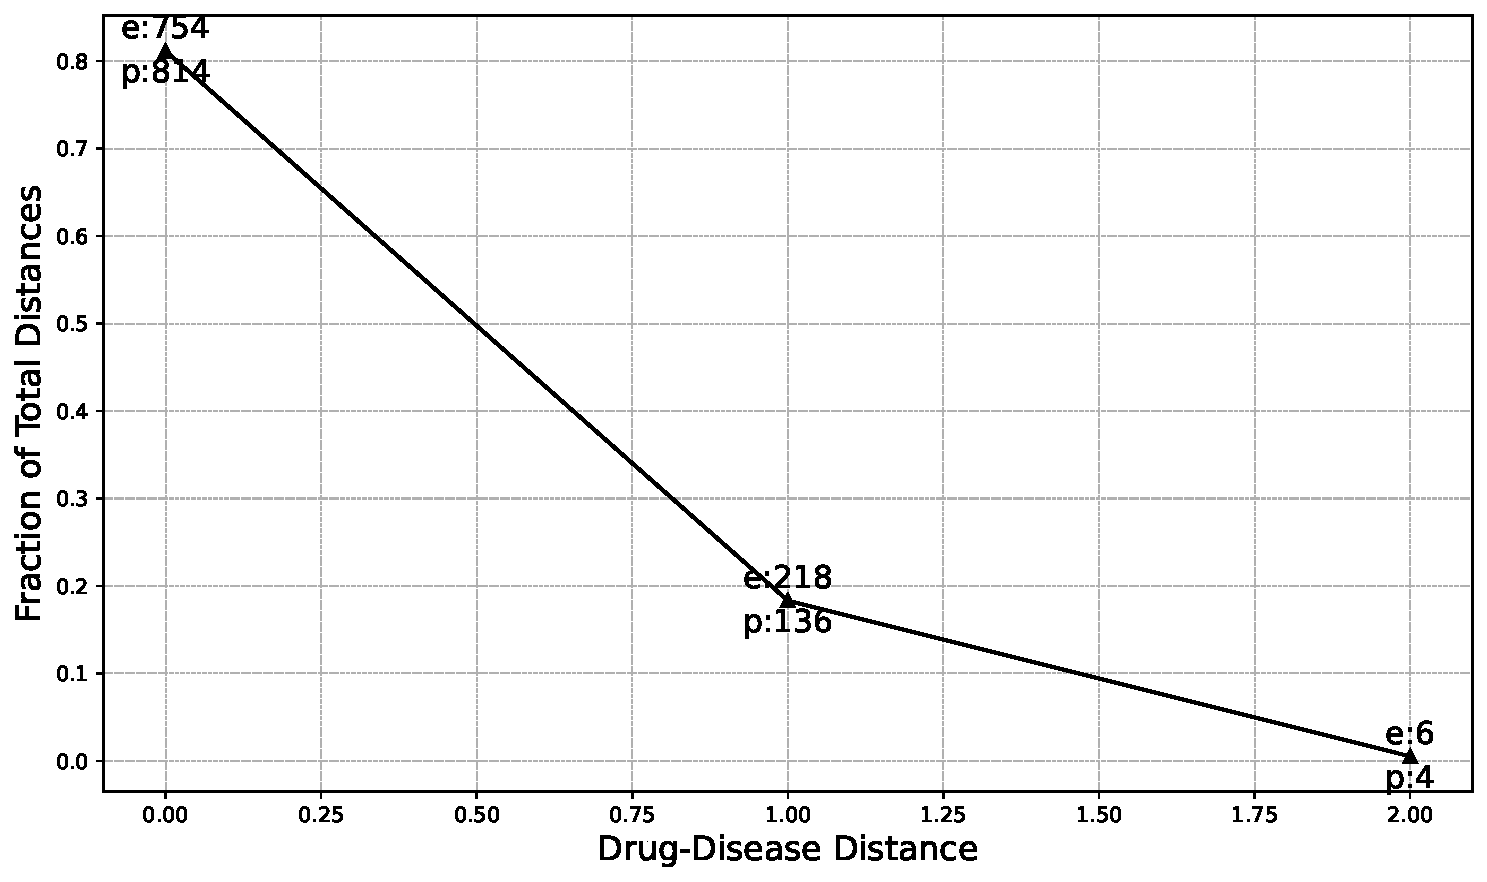
\includegraphics[width=\linewidth]{Figures/Yildrim_unique_minimum_shortest_distance.pdf}
   \caption{\textbf{Unique Minimum Shortest Distance Method:} 
   For each drug, we identified its shortest distance to a disease. 
   If a drug had the same shortest distance to multiple diseases, we retained only one unique distance per drug, removing duplicates.
   }
   \label{fig:yildirim3}
\end{subfigure}
\caption{Three methods for calculating drug-disease distances.
%We refer to the methodology of \cite{yildirim2007drug}.
Abbreviations: e = Etiological, p = Palliative. 
Numerical values represent the number of paths between drug and disease pairs at a specific distance. 
The fraction for each distance (path length) is calculated by dividing the number of occurrences of that specific path length by the total number of paths in the dataset.
This measures how common each distance is, relative to all possible paths.}
\label{fig:yildirim}
\end{figure}

%\end{appendices}

\end{document}
